% ****** Start of file apssamp.tex ******
%
%   This file is part of the APS files in the REVTeX 4.2 distribution.
%   Version 4.2a of REVTeX, December 2014
%
%   Copyright (c) 2014 The American Physical Society.
%
%   See the REVTeX 4 README file for restrictions and more information.
%
% TeX'ing this file requires that you have AMS-LaTeX 2.0 installed
% as well as the rest of the prerequisites for REVTeX 4.2
%
% See the REVTeX 4 README file
% It also requires running BibTeX. The commands are as follows:
%
%  1)  latex apssamp.tex
%  2)  bibtex apssamp
%  3)  latex apssamp.tex
%  4)  latex apssamp.tex
%
\documentclass[%
 reprint,
%superscriptaddress,
%groupedaddress,
%unsortedaddress,
%runinaddress,
%frontmatterverbose, 
%preprint,
%preprintnumbers,
%nofootinbib,
%nobibnotes,
%bibnotes,
 amsmath,amssymb,
 aps,
 pra,
%prb,
%rmp,
%prstab,
%prstper,
%floatfix,
]{revtex4-2}
\usepackage[spanish,es-nodecimaldot]{babel}
\usepackage{color,soul}
\usepackage{physics}
\usepackage{minted}
\usepackage{graphicx}% Include figure files
%\usepackage{svg}
\usepackage{dcolumn}% Align table columns on decimal point
\usepackage{bm}% bold math
\usepackage{hyperref}% add hypertext capabilities
\definecolor{linkcolour}{rgb}{0,0.2,0.6} % Link color
\hypersetup{colorlinks,citecolor=linkcolour,breaklinks,urlcolor=linkcolour,linkcolor=linkcolour}
\usepackage{color,soul}
\usepackage{soulutf8}
%\usepackage[mathlines]{lineno}% Enable numbering of text and display math
%\linenumbers\relax % Commence numbering lines

%\usepackage[showframe,%Uncomment any one of the following lines to test 
%%scale=0.7, marginratio={1:1, 2:3}, ignoreall,% default settings
%%text={7in,10in},centering,
%%margin=1.5in,
%%total={6.5in,8.75in}, top=1.2in, left=0.9in, includefoot,
%%height=10in,a5paper,hmargin={3cm,0.8in},
%]{geometry}

\begin{document}

\preprint{APS/123-QED}

\title{Oscilador armónico cuántico unidimensional en baño\\térmico usando el algoritmo Metrópolis.}% Force line breaks with \\

\author{Juan Esteban Aristizabal Zuluaga}
\affiliation{Instituto de Física, Universidad de Antioquia.}%Lines break automatically or can be forced with \\

\date{\today}% It is always \today, today,
             %  but any date may be explicitly specified

\begin{abstract}
En este artículo presentamos un estudio del oscilador armónico cuántico unidimensional en un baño térmico. En particular, nos interesamos por calcular la probabilidad de encontrar el sistema en una posición dada. Para esto, presentamos los cálculos teóricos cuánticos y su contraparte clásica, con el fin de comparar los resultados. Especialmente nos enfocamos en usar el algoritmo Metrópolis para reconstruir histogramas que representan las distribuciones de probabilidad cuánticas, tanto en el espacio de posiciones como en los niveles de energía. Estos resultados cuánticos los usamos para contrastarlos con los clásicos y los tres casos presentados   –baja, media y alta temperatura– concuerdan claramente con los cálculos teóricos. Se presenta también la implementación del algoritmo Metrópolis en el lenguaje de programación «Python». 
\begin{description}
\item[Palabras clave] 	Oscilador armónico, física estadística cuántica, baño térmico, ensamble \\
						canónico, algoritmo Montecarlo.
\end{description}
\end{abstract}

%\keywords{Suggested keywords}%Use showkeys class option if keyword
                              %display desired
\maketitle

%\tableofcontents

\section{\label{sec:Intro}Introducción}
El oscilador armónico ha sido históricamente para la física un sistema simple pero del que se puede extraer gran cantidad de información y con el que se han descubierto muchos nuevos métodos y hasta teorías completas, basadas en los razonamientos y el conocimiento obtenido de éste. Por citar un ejemplo, está la cuantización del campo electromagnético que se puede reducir a un sistema «osciladores armónicos» no acoplados y en general las teorías de segunda cuantización en la base número usan gran parte del formalismo del oscilador armónico cuántico, aunque con un significado muy diferente al que se le da en el sistema que nos compete\cite{Grynberg2010,Schwartz2013}. 

En nuestro caso hemos tomado el oscilador armónico unidimensional inmerso en un baño térmico y hemos estudiado su comportamiento a diferentes temperaturas y contrastado los resultados cuántico y clásico para la probabilidad de encontrarlo en una posición dada. Para ello hemos revisado los resultados teóricos. Entre diferentes alternativas presentadas en la literatura para llegar al resultado cuántico, entre ellas el formalizmo de intrgrales de camino \cite{Barone2003,Holstein1998}, propagadores \cite{Kheirandish2018}  y métodos más heurísticos como el de Feynman \cite{RichardP.Feynmann1972}, hemos decidido presentar el formalismo desarrollado por Cohen-Tannoudji \cite{Cohen-Tannoudji}, el cual deriva una ecuación diferencial parcial para encontrar los elementos de matriz diagonales del operador densidad, los cuales corresponden con la probabilidad en la que estamos interesados. El método que presentamos tiene la ventaja de que requiere de cálculos básicos y no de métodos avanzados, que pueden ser un poco más confusos.

Por otro lado, como sabemos, en la física estadística las herramientas computacionales han permitido un mejor entendimiento de diversos problemas. En particular, el algoritmo Metrópolis ha sido ámpliamente usado desde que  Metropolis \textit{et al.} publicaron el artículo que lo propone \cite{Metropolis1953}, en el año 1953, que posteriormente gananó más popularidad con la generalización hecha en 1970 por Hastings \cite{Hastings1970}. El algoritmo es útil especialmente en problemas de alta dimensionalidad para muestrear distribuciones de probabilidad en el que otros métodos no son igual de eficientes o simplemente no funcionan –uno de los ejemplos más comunes es la implementación de este algoritmo en sistemas tipo Ising \cite{Newman1999}–, aunque en teoría se puede usar para sistemas con cualquier dimensionalidad. 

En nuestro caso, a pesar de tener un sistema de baja dimensionalidad, usamos el algoritmo metrópolis para obtener los histogramas de las densidades de probabilidad para el caso cuántico tanto para $T=0$ como varios valores de $T \neq 0$.  Por otro lado, usando el mismo algoritmo, encontramos histogramas para los niveles de energía en cada caso y comprobamos que corresponden con la distribución de Boltzmann \textit{i.e.} la distribución de probabilidad dada por el ensamble canónico de la física estadística.

La estructura del artículo es la siguiente: en la sección \ref{sec:Teoria} presentamos los resultados teóricos para la densidad de probabilidad cuántica y clásica de encontrar el oscilador armónico unidimensional en una posición dad cuando éste está inmerso en un baño térmico. En la parte \ref{sec:Resultados} contrastamos los resultados teóricos clásico y cuántico con simulaciones usando el algoritmo Montecarlo para la parte cuántica, para diferentes valores de temperatura. En esta sección también comprobamos los resultados y los límites de alta y baja temperatura que obtuvimos en \ref{sec:Teoria}. En \ref{sec:conclusion} presentamos la conclusión del trabajo y, finalmente, en los apéndices \ref{appx:codigo_baja_temperatura} y \ref{appx:codigo_temperatura_finita} escribimos las implementaciones de los algoritmos de metrópolis usados (en Python3) para generar las figuras y para los análisis de la sección \ref{sec:Resultados}. 


\section{\label{sec:Teoria}Consideraciones teóricas}

Consideraremos los sistemas en unidades reducidas, es decir, con sus variables adimensionalizadas.


\subsection{Caso Clásico} \label{subsec:caso-clasico}
Queremos encontrar la densidad de probabilidad de que una partícula en un potencial armónico unidimensional y en un baño térmico a temperatura $T = 1/\beta$ se encuentre en la posición x. Esta densidad de probabilidad se encuentra al integrar todas las contribuciones de los diferentes momentos de la partícula:
\begin{equation}
	\pi^{(C)}(x;\beta) = \int_{-\infty}^\infty dp \rho(p,x;\beta),  \label{eq:Classical-probability}
\end{equation}
donde $\rho(p,x;\beta)$ es la densidad de probabilidad clásica –en el espacio de fase– del ensamble canónico que está dada por
\begin{equation}
	\rho(p,x;\beta) = \exp[-\beta H(p,x)] / Z(\beta) ,  \label{eq:Classical-Ensemble}
\end{equation}
donde
\begin{equation}
	Z(\beta) = \int_{-\infty}^\infty \int_{-\infty}^\infty dp dx \exp[-\beta H(p,x)]
\end{equation} 
es la función de partición canónica.
En nuestro caso, para el oscilador armónico tenemos que el hamiltoniano está dado por
\begin{equation}
	H(p,x) = \frac{1}{2} p^2 + \frac{1}{2} x^2. \label{eq:Classical-Hamiltonian}
\end{equation}
La función de partición canónica está dada por
\begin{eqnarray}
	Z(\beta) 	&=& \int_{-\infty}^\infty \int_{-\infty}^\infty dp dx \exp[-\beta \left( \frac{p^2}{2} + \frac{x^2}{2} \right) ] \\ 
				&=& \frac{2}{\beta} \int_{-\infty}^\infty dy e^{-y^2} \int_{-\infty}^\infty dz e^{-z^2} \nonumber \\
				&=& \frac{2\pi}{\beta},
\end{eqnarray}
donde usamos los cambios de variable $\frac{\beta}{2}p^2 \rightarrow y^2$ $\frac{\beta}{2}x^2 \rightarrow z^2$ y el resultdo de la integral gaussiana $\int_{-\infty}^\infty dz e^{-z^2} = \sqrt{\pi}$. De este resultado y de la ec. (\ref{eq:Classical-Ensemble}) obtenemos para el oscilador armónico
\begin{equation}
	\rho(p,x;\beta) = \frac{\beta}{2\pi} \exp[-\beta \left( \frac{p^2}{2} + \frac{x^2}{2} \right) ] \label{eq:HO-Classical-Ensemble}.
\end{equation}
Usando la ec. anterior en (\ref{eq:Classical-probability}) obtenemos la probabilidad que buscábamos 
\begin{align}
	\pi^{(C)}(x;\beta) =& \frac{\beta}{2\pi}\int_{-\infty}^\infty dp \exp[-\beta \left( \frac{p^2}{2} + \frac{x^2}{2} \right)] \nonumber \\
	=&\frac{\beta}{2\pi}e^{-\beta x^2/2}
	\int_{-\infty}^\infty dp e^{-\beta p^2/2} \nonumber
\end{align}
\begin{equation}
	\!\!\!\!\!\!\!\!\!\!\!\!\!\!\!\!\!\!\!\!\!\!\! \iff \pi^{(C)}(x;\beta) = \sqrt{\frac{\beta}{2\pi}}e^{-\beta x^2/2} \label{eq:pi-classical-finale}
\end{equation}

Si comparamos nuestro resultado (\ref{eq:pi-classical-finale}) con la famosa PDF gaussiana, encontramos que su varianza está dada por
\begin{equation}
	\sigma^2 = \frac{1}{\beta} = T.
\end{equation}

Notando esto es fácil analizar qué pasará en el caso clásico en los límites de altas y bajas temperaturas. En el primer caso, tenemos que la varianza de nuestra densidad de probabilidad sería inmensa. La probabilidad de encontrar a la partícula tiende a una distribución uniforme y si estamos trabajando en un espacio infinito $x\in(-\infty,\infty)$, en el límite $T\rightarrow\infty$ la probabilidad de encontrar a la partícula en un punto determinado sería efectivamente cero.

Por otro lado, en el límite de bajas temperaturas, la varianza de la probabilidad es tan baja como la temperatura misma. Es decir, a medida que bajamos la temperatura, el ancho de nuestra distribución gaussiana disminuye también. Esto implica que la probabilidad de encontrar la «partícula» en el centro del potencial \textit{i.e.} en $x=0$ aumenta conforme $T$ disminuye, hasta que en el límite $T\rightarrow 0$ la probabilidad de encontrarla en dicho punto es uno. Es decir, la partícula permanece inmóvil en dicho sitio. En términos matemáticos, decimos que la distribución de probabilidad en este límite es una delta de Dirac centrada en el mínimo del potencial.

\subsection{Caso cuántico} \label{subsec:caso-cuantico}
En el caso cuántico, para calcular la densidad de probabilidad de encontrar a la parícula en la posición $x$ seguiremos a Cohen-Tannoudji \cite{Cohen-Tannoudji}. Primero, recordemos que en este caso el operador densidad en el ensamble canónico está dado por
\begin{equation}
	\hat{\rho} = \exp[-\beta \hat{H}].
\end{equation}
De este modo es claro que la normalización de $\hat{\rho}$ está dada por la función de partición canónica
\begin{equation}
	Z(\beta) = \Tr[\hat{\rho}]=\sum_n e^{-\beta E_n}\label{eq:Quantum-Z}
\end{equation} 
Donde $\{E_n\}_n$ son los niveles de energía del sistema y $n$ es un índice colectivo de números cuánticos que caracterizan el espectro de $\hat{H}$. En caso de que dicho espectro sea continuo, la suma en la expresión anterior se debería cambiar por una integral sobre las energías o los índices continuos que caracterizan las energías. 

La densidad de probabilidad que se busca es
\begin{equation}
	\pi^{(Q)}(x;\beta) = \rho(x,x;\beta)/Z(\beta) = \ev{\hat{\rho}}{x}/Z(\beta). \label{eq:Quantum-pi}
\end{equation}

En nuestro caso el hamiltoniano está dado por
\begin{equation}
	\hat{H} = \frac{1}{2} \hat{p}^2 + \frac{1}{2} \hat{x}^2. \label{eq:Quantum-Hamiltonian}
\end{equation}
Los autoestados de energía están dados por $\{\ket{n}\}_n$, donde $n\in\{0,1,2,3,...\}$ y sus autovalores están dados por 
\begin{equation}
	\hat{H}\ket{n} = \left(n+\frac{1}{2}\right)\ket{n}.
\end{equation}
es decir, $E_n = n+1/2$.

Con el valor de $E_n$ y la ecuación (\ref{eq:Quantum-Z}) podemos calcular ahora el valor de la función de partición
\begin{eqnarray}
	Z(\beta) 	&=& e^{-\beta/2}\sum_n e^{-\beta n}    \nonumber\\
				&=&  e^{-\beta/2}\sum_n \left( e^{-\beta } \right)^n  \nonumber\\
				&=&  \frac{e^{-\beta/2}}{1 - e^{-\beta}} \nonumber \\
				&=& \frac{1}{2\sinh(\beta/2)}.
\end{eqnarray}
Donde en la tercera igualdad hemos usado que $0<e^{-\beta}<1$ y el resultado de la serie geométrica $\sum_{n=0}^\infty a^n = 1/(1-a)$ si $|a|<1$

Por otro lado, como sabemos, el hamiltoniano del oscilador armónico puede ser escrito en términos de los operadores escalera $a$ y $a^\dag$, que están definidos como
\begin{eqnarray}
	a &=& \frac{1}{\sqrt{2}}\left(\hat{x}+i\hat{p}\right) \label{eq:ladder-down}\\ 
	a^\dag &=& \frac{1}{\sqrt{2}}\left(\hat{x}-i\hat{p}\right) \label{eq:ladder-up},
\end{eqnarray}
y que tienen las siguientes propiedades
\begin{eqnarray}
	\left[ a, a^\dag \right] 	&=& 1 \\
								a\ket{n} &=& \sqrt{n}\ket{n-1} \label{eq:ladder-down-on-ket}\\
								a^\dag\ket{n} &=& \sqrt{n+1}\ket{n+1}\\
								a^\dag a\ket{n} &=& n\ket{n+1} \label{eq:number-on-ket}. 
\end{eqnarray}

Se encuentra que 
\begin{equation}
	H = a^\dag a+\frac{1}{2}.
\end{equation}

Con este formalismo en mente, nuestro objetivo ahora es encontrar el elemento de matriz $\ev{\hat{\rho}}{x}$ para así poder calcular la probabilidad $\pi(x;\beta)$ definida en (\ref{eq:Quantum-pi}). Tenemos
\begin{eqnarray}
	\ev{\hat{\rho}}{x}	&=& \ev{e^{-\beta\left(a^\dag a + 1/2\right)}}{x} \nonumber \\
						&=& e^{-\beta/2}F_\beta(x) \label{eq:rho_x_x},
\end{eqnarray}
donde hemos definido
\begin{equation}
	F_\beta(x) = \ev{e^{-\beta a^\dag a}}{x}.
\end{equation}

Para evaluar el elemento de matriz $F_\beta(x)$ encontraremos una ecuación diferencial que lo caracterice, usando el formalismo de las transformaciones unitarias infinitesimales. Recordemos que como $\hat{p}$ es el generador de las traslaciones
\begin{equation}
	\ket{x+dx} = \left( 1 - i \hat{p} dx \right)\ket{x},
\end{equation}
por tanto, tenemos que
\begin{eqnarray}
	F_\beta(x+dx) 	&=& \ev{e^{-\beta a^\dag a}}{x+dx} \nonumber \\ 
					&=& \ev{\left( 1 + i \hat{p} dx \right)e^{-\beta a^\dag a}\left( 1 - i \hat{p} dx \right)}{x} \nonumber \\
					&=& F_\beta(x)+idx\ev{\hat{p}e^{-\beta a^\dag a} - e^{-\beta a^\dag a}\hat{p}}{x} \nonumber \\
					&=& F_\beta(x)+idx\ev{\left[\hat{p},e^{-\beta a^\dag a}\right]}{x}
\end{eqnarray}
Donde en la tercera igualdad se ignoran términos de orden $(dx)^2$, ya que estamos considerando desplazamientos infinitesimales. Por tanto, de lo anterior obtenemos la expresión
\begin{equation}
	\frac{F_\beta(x+dx)-F_\beta(x)}{dx} = i\ev{\left[\hat{p},e^{-\beta a^\dag a}\right]}{x},
\end{equation}
y tomando $\lim_{dx\rightarrow0}$ obtenemos la ecuación diferencial deseada
\begin{equation} 
	\frac{d}{dx}F_\beta(x) = i\ev{\left[\hat{p},e^{-\beta a^\dag a}\right]}{x}. \label{eq:Diff-Eqn-F(x)}
\end{equation}

Ahora nuestro problema se concentra en calcular el elemento de matriz $\ev{\left[\hat{p},e^{-\beta a^\dag a}\right]}{x}$. Para esto calcularemos primero una expresión quivalente a la del conmutador, que facilitará el cálculo. Notamos de las ecuaciones (\ref{eq:ladder-down}) y (\ref{eq:ladder-up}) que $\hat{p} = \frac{1}{i\sqrt{2}}\left(a-a^\dag\right)$. Por tanto, tenemos que
\begin{eqnarray}
	\left[\hat{p},e^{-\beta a^\dag a}\right] 	&=& \frac{1}{i\sqrt{2}}\left[a-a^\dag,e^{-\beta a^\dag a}\right]. \label{eq:commutator}
\end{eqnarray}
El conmutador en la expresión anterior involucra a $a-a^\dag$, pero quisiéramos obtener una relación que involucre a $a+a^\dag$ que, según las expresiones (\ref{eq:ladder-down}) y (\ref{eq:ladder-up}), es proporcional a $\hat{x}$ y actua de manera simple en los kets $\ket{x}$ de la expresión (\ref{eq:Diff-Eqn-F(x)}). Para lograr ésto examinaremos la relación entre los términos $a e^{-\beta a^\dag a}$ y $e^{-\beta a^\dag a}a$. Dicha relación es evidente si consideramos sus elementos de matriz en la representación $\{\ket{n}\}_n$. Tenemos
\begin{eqnarray}
	\mel{m}{a e^{-\beta a^\dag a}}{n} 	&=& \sqrt{n}e^{-\beta n} \braket{m}{n-1} \nonumber \\
										&=&  \sqrt{n}e^{-\beta n} \delta_{m,\,n-1}, \label{eq:mel-1}
\end{eqnarray}
y
\begin{eqnarray}
	\mel{m}{e^{-\beta a^\dag a} a}{n} 	&=& \sqrt{n}e^{-\beta (n-1)} \braket{m}{n-1} \nonumber\\
										&=&  \sqrt{n}e^{-\beta (n-1)} \delta_{m,\,n-1}. \label{eq:mel-2}
\end{eqnarray}
De (\ref{eq:mel-1}) y (\ref{eq:mel-2}) deducimos 
\begin{equation}
	e^{-\beta a^\dag a} a = e^\beta a e^{-\beta a^\dag a}.
\end{equation}
Es fácil ver que la expresión anterior es equivalente a
\begin{equation}
	\left(1-\tanh\frac{\beta}{2}\right)e^{-\beta a^\dag a} a = \left(1+\tanh\frac{\beta}{2}\right) a e^{-\beta a^\dag a}. \label{eq:relation-a-times-exp}
\end{equation}
Similarmente, tenemos
\begin{eqnarray}
	\mel{m}{a^\dag e^{-\beta a^\dag a}}{n} 	&=& \sqrt{n+1}e^{-\beta n} \braket{m}{n+1} \nonumber \\
										&=&  \sqrt{n+1}e^{-\beta n} \delta_{m,\,n+1} \label{eq:mel-3}
\end{eqnarray}
y
\begin{eqnarray}
	\mel{m}{e^{-\beta a^\dag a }a^\dag}{n} 	&=& \sqrt{n+1}e^{-\beta (n+1)} \braket{m}{n+1} \nonumber\\
											&=&  \sqrt{n+1}e^{-\beta (n+1)} \delta_{m,\,n+1} \label{eq:mel-4}
\end{eqnarray}
y por tanto, tenemos que
\begin{equation}
	e^{-\beta a^\dag a} a^\dag = e^{-\beta} a^\dag e^{-\beta a^\dag a}, 
\end{equation}
y esta expresión es equivalente a 
\begin{equation}
	\left(1+\tanh\frac{\beta}{2}\right)e^{-\beta a^\dag a} a^\dag = \left(1-\tanh\frac{\beta}{2}\right) a^\dag e^{-\beta a^\dag a}.\label{eq:relation-adag-times-exp}
\end{equation}

Restando las expresiones (\ref{eq:relation-a-times-exp}) y (\ref{eq:relation-adag-times-exp}) obtenemos 
\begin{align}
	e^{-\beta a^\dag a}&\left(a -a^\dag \right)-\tanh\frac{\beta}{2}e^{-\beta a^\dag a}\left(a +a^\dag \right)  = \nonumber \\
	&  \left(a -a^\dag \right)e^{-\beta a^\dag a}+\tanh\frac{\beta}{2}\left(a + a^\dag \right)e^{-\beta a^\dag a}.
\end{align}
Reorganizando los términos, encontramos que
\begin{equation}
	\left[a-a^\dag,e^{-\beta a^\dag a}\right] = - \tanh\frac{\beta}{2} \left[a+a^\dag,e^{-\beta a^\dag a}\right]_+
\end{equation}
donde $[A,B]_+ = AB+BA$. Además, de las relaciones (\ref{eq:ladder-down}) y (\ref{eq:ladder-up}) sabemos que $\hat{x}=\left( a+a^\dag \right)/\sqrt{2}$ y por tanto, la expresión anterior se puede escribir como
\begin{equation}
	\left[a-a^\dag,e^{-\beta a^\dag a}\right] = - \sqrt{2}\tanh\frac{\beta}{2} \left[\hat{x},e^{-\beta a^\dag a}\right]_+ \label{eq:commutator-in-terms-of-x}
\end{equation}
Remplazando la expresión anterior en (\ref{eq:commutator}) obtenemos
\begin{equation}
	\left[\hat{p},e^{-\beta a^\dag a}\right] = i\tanh\frac{\beta}{2} \left[ \hat{x} , e^{-\beta a^\dag a} \right]_+.
\end{equation}
Remplazando ésta última expresión en la ecuación diferencial para $F_\beta(x)$, (\ref{eq:Diff-Eqn-F(x)}), encontramos que
\begin{align}
	\frac{d}{dx} F_\beta(x)	&= -\tanh \frac{\beta}{2} \ev{ \left[ \hat{x} , e^{-\beta a^\dag a} \right] _+ }{x} \nonumber \\
							&= -\tanh \frac{\beta}{2} \ev{ \left( \hat{x} e^{-\beta a^\dag a} + e^{-\beta a^\dag a} \hat{x} \right)}{x} \nonumber \\
							&= -\tanh(\frac{\beta}{2}) 2 x  \ev{e^{-\beta a^\dag a}}{x} \nonumber \\
	\iff	 \frac{d}{dx}  F_\beta(x)& + \tanh(\frac{\beta}{2}) 2 x F_\beta(x) = 0
\end{align}
es fácil ver que la ecuación diferencial obtenida es de la forma $g'(x) + \frac{2x}{\zeta^2}g(x) = 0$ y que la solución de esta ecuación es una gaussiana $g(x)=c_0 e^{-x^2/\zeta^2}$ donde $c_0$ está definida por una condición inicial. En nuestro caso $ 1 / \zeta^2 = \tanh(\beta/2)$. Por tanto tenemos que
\begin{equation}
	F_\beta(x) = c_0 \exp[-\tanh(\beta/2)x^2].
\end{equation}

Remplazando el resultado anterior en  (\ref{eq:rho_x_x}) encontramos que $\ev{\hat{\rho}}{x}= c_0e^{-\beta/2}\exp[-\tanh(\beta/2)x^2]$ y remplazando este resultado en (\ref{eq:Quantum-pi}) encontramos que la probabilidad (densidad) que buscábamos está dada por
\begin{equation}
	\pi^{(Q)}(x;\beta) = c_0e^{-\beta/2}\exp[-\tanh(\beta/2)x^2]/Z(\beta)
\end{equation}

Finalmente, sabemos que al ser $\pi(x;\beta)$ una densidad de probabilidad, su integral debe ser igual a uno. Usando este hecho y el resultado de la integral gausiana dado en la sección \ref{subsec:caso-clasico}, encontramos que $c_0 e^{-\beta/2}/Z(\beta)=\sqrt{\tanh(\beta/2)/\pi}$, es decir, en el ensamble canónico la probabilidad (densiadad) de encontrar a la partícula en la posición $x$ está dada por
\begin{equation}
	\pi^{(Q)}(x;\beta) = \sqrt{\frac{\tanh(\beta/2)}{\pi}}\exp[-\tanh(\beta/2)x^2]. \label{eq:pi-quantum-finale}
\end{equation}


Analizar los límites de la expresión (\ref{eq:pi-quantum-finale}) también es sencillo. En el caso de bajas temperatura tenemos que $\beta \gg 1$ y por tanto $\tanh(\beta/2)\rightarrow 1$ y la densidad de probabilidad límite es $\pi^{(Q)}(x,\beta\gg 1) \approx e^{-x^2}/\sqrt{\pi}$. Este resultado corresponde con la densidad de probabilidad del estado base del oscilador armónico, $|\psi_0(x)|^2$  donde 
\begin{equation}
	\psi_0(x) = \frac{1}{\pi^{1/4}} e^{-x^2/2},	\label{eq:QHO-ground-state}
\end{equation}
conforme esperábamos: en el límite de bajas temperaturas los sistemas cuánticos tienden a ocupar su estado base.

Por otro lado, en el límite de altas temperaturas esperamos obtener el caso clásico. De hecho, para este límite tenemos $\beta \ll 1$ lo cual implica $\tanh(\beta/2)\rightarrow\beta/2$ y obtenemos la densidad de probabilidad clásica, $\pi^{(Q)}(x;\beta \ll 1) \approx \sqrt{\beta/2\pi}e^{-\beta x^2/2}$, que corresponde con el resultado (\ref{eq:pi-classical-finale}).

Es interesante ver que en este ejemplo se manifiesta de manera sencilla el hecho de que en el caso de sistemas en equilibrio con reservorios de calor, los efectos de la mecánica cuántica son más evidentes en el límite de bajas temperaturas, en el cual los resultados cuántico y clásico son completamente diferentes.

Como dijimos al comienzo de esta sección, las cantidades que tratamos acá son adimensionales. Sin embargo, si queremos pasar a un sistema físico particular que se pueda reducir a un oscilador armónico en un baño térmico, en el caso cuántico podemos hacer el cambio $\beta\rightarrow\hbar\omega / k_B T$ para tener una idea de las dimensiones y casos de alta temperatura  ($T \gg \hbar\omega / k_B$) o de baja temperatura ($T \ll \hbar\omega / k_B$) con valores particulares según sea el sistema considerado. En el caso clásico este paso se puede hacer haciendo el cambio $\beta \rightarrow m\omega^2l_0^2/k_B T$, donde $l_0$ es una longitud característica del sistema y $m$ es la masa de la «partícula».


\section{\label{sec:Resultados}Resultados y discusión}
A continuación presentaremos los resultados del límite de baja temperatura para un oscilador armónico cuántico unidimensional y su contraparte clásica y de igual forma para temperaturas por encima de $T \rightarrow 0$, en el marco de simulaciones que usan cadenas de Markov en el algoritmo Metropolis. Como ya se mencionó en la Sección \ref{sec:Intro}, éste algoritmo permite realizar un muestreo de la densidad de probabilidad (\ref{eq:pi-quantum-finale}), hallada en la Sección \ref{sec:Teoria}. Las implementaciones de los algoritmos en el lenguaje de programación Python3 se pueden ver en los apéndices \ref{appx:codigo_baja_temperatura} y \ref{appx:codigo_temperatura_finita}.

\subsection{Límite de muy baja temperatura \texorpdfstring{$T \rightarrow 0$}{T tendiendo a cero}\label{subsec:limite-T-0}}

En el caso clásico y el límite de muy baja temperatura ($T \rightarrow 0 $), según discutimos en la sección \ref{subsec:caso-clasico}, la densidad de probabilidad de encontrar la «partícula» en la posición $x$ tiende a una delta de Dirac: $\pi^{(C)}(x;\beta \gg 1) \rightarrow \delta(x)$. En la figura \ref{fig:classic_probability} encontramos $\pi^{(C)}(x;\beta)$ para diferentes valores de $\beta$, cada vez más grandes y podemos ver que para valores altos de $\beta$ (temperaturas bajas) la distribución comienza a tener el límite mencionado. Aunque es solo una aproximación gráfica, podemos ver que ilustra muy bien el límite.
\begin{figure}[!t]
	\centering
	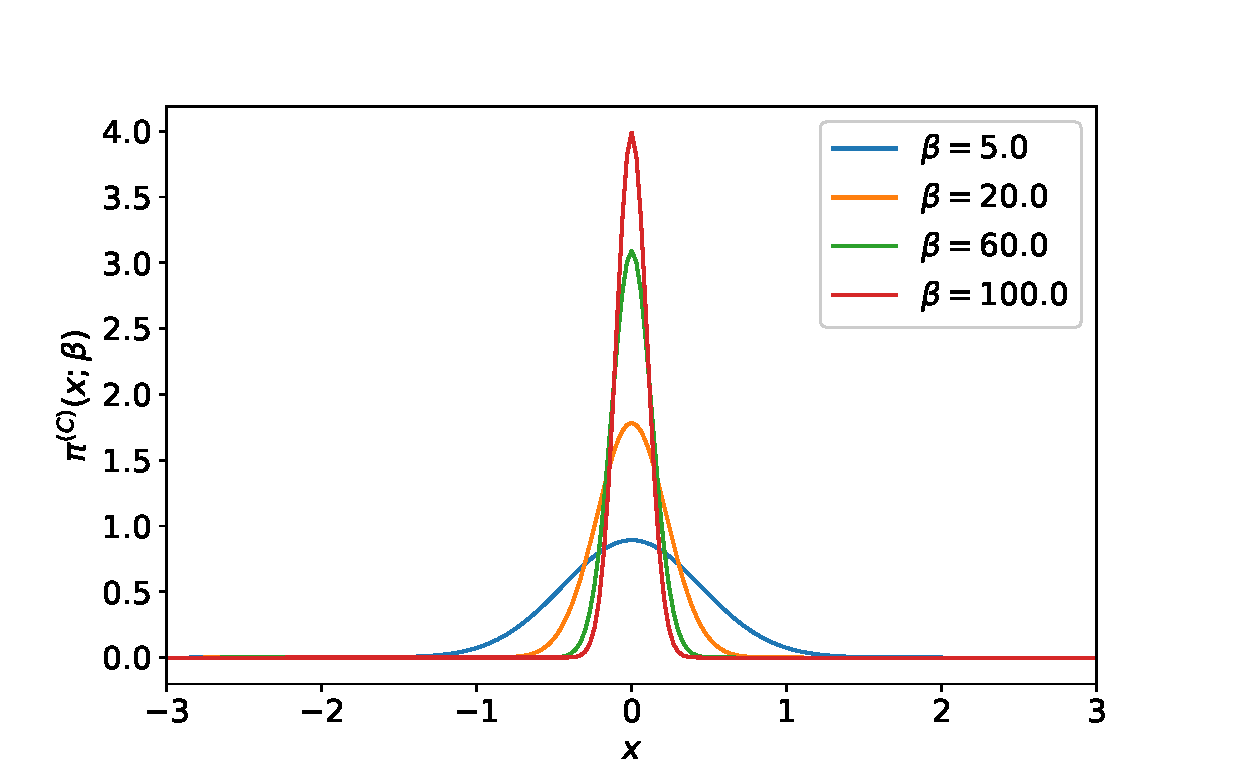
\includegraphics[width=\linewidth]{figures/plot_CHO_finite_temp_several_beta}
	\caption{Probabilidad de encontrar a la partícula clásica en presencia de un potencial armónico en una posición $x$, cuando ésta se encuentra en un reservorio de Calor a temperatura $T=1/\beta$. Se ilustra gráficamente el hecho de que $\pi^{(C)}(x;\beta) \rightarrow \delta(x)$ cuando $\beta\rightarrow\infty$.}
	\label{fig:classic_probability}
\end{figure}

El límite de muy baja temperatura para el caso cuántico, como se discutió en la sección \ref{subsec:caso-cuantico}, es que la densidad de probabilidad $\pi^{(Q)}(x;\beta)$ tiende a la misma densidad de probabilidad del estado base del sistema, la cual determinada por la norma al cuadrado de $\psi_0(x)$, (\ref{eq:QHO-ground-state}). En este caso usamos el algoritmo Metrópolis solo para muestrear posiciones de la distribución de probabilidad definoda por $|\psi_0(x)|$, ya que en este límite los niveles excitados del sistema no son accesibles o su accesibilidad es despreciable. 

\begin{figure}[!t]
	\centering
	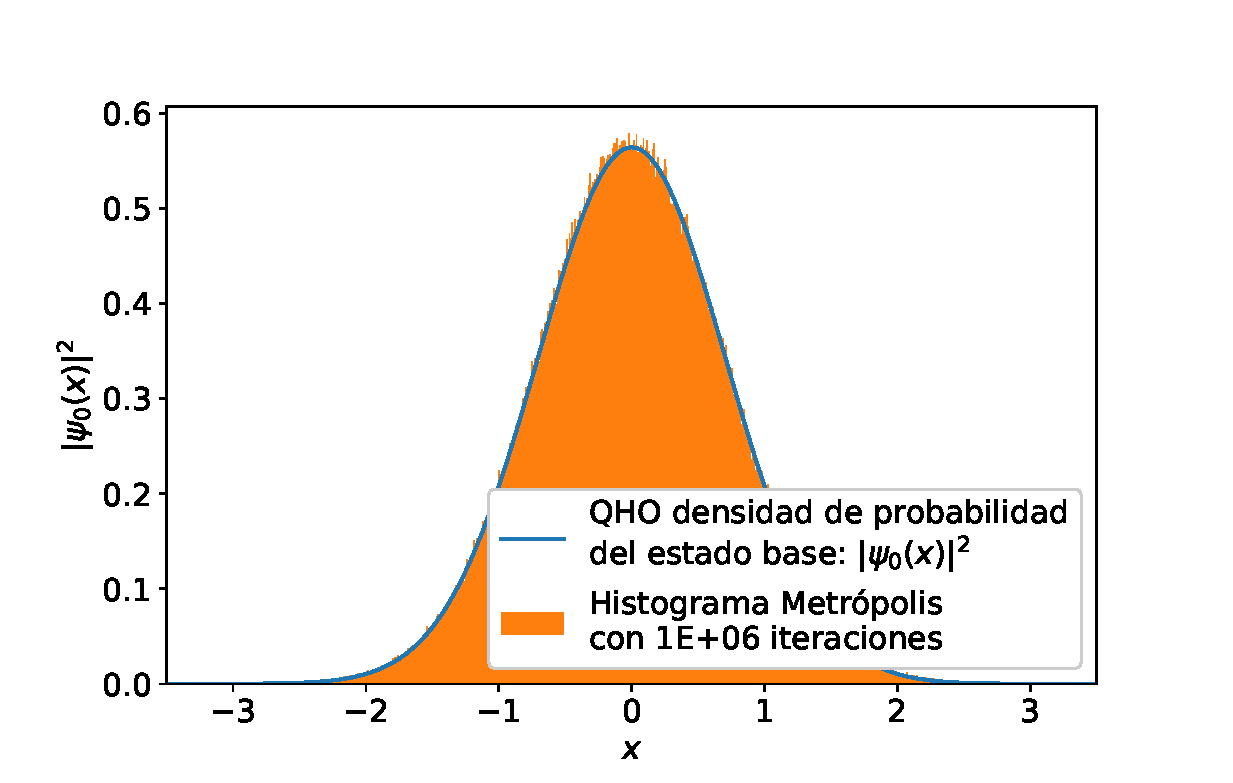
\includegraphics[width=\linewidth]{figures/plot_QHO_ground_state}
	\caption{Densidad de probabilidad de encontrar a la «partícula» cuántica en una posición dada, cuando está en presencia de un potencial armónico y en ausencia de baño térmico \textit{i.e.} $T=0$ . Se muestra el resultado teórico como línea continua y el histograma que resulta del algoritmo Metrópolis.}
	\label{fig:ground_state}
\end{figure}

En la figura \ref{fig:ground_state} mostramos la densidad de probabilidad teórica para el estado base, $|\psi_0(x)|^2$, y el histograma que obtenemos mediante el algoritmo de Metrópolis, cuya implementación se puede revisar en el apéndice \ref{appx:codigo_baja_temperatura}. Para obtener esta gráfica usamos $10^6$ iteraciones en el algoritmo y para la propuesta de la posición en cada nueva iteración se usó una distribución uniforme centrada en el valor de $x$ de la iteración inmediatamente anterior: $x_{new} \sim U(x_{old} - \delta x, x_{old} + \delta x)$. En este caso se usó $\delta x = 0.5$. La probabilidad de aceptación de la proposición es de
\begin{equation}
	p(x_{old} \rightarrow x_{new}) = \min\left(1,\left|\frac{\psi_{0}(x_{new})}{\psi_{0}(x_{old})}\right|^2\right).
\end{equation}
Podemos ver que el resultado de este ejercicio es satisfactorio. Encontramos que el histograma corresponde en gran medida con la densidad de probabilidad teórica, lo cual implica que el muestreo –a pesar de que es posible que no sea el más óptimo– si está bien realizado.

\subsection{Temperatura finita \texorpdfstring{$T \neq 0$}{T diferente de cero}\label{subsec:temperatura-finita}}
Para temperaturas $T\neq0$ el oscilador armónico ahora puede acceder a niveles de energía diferentes del nivel de energía base  ($n=0$). Es por esto que la implementación del algoritmo Metrópolis en este caso debe tener en cuenta tanto cambios de posición como cambios en los niveles de energía. En la implementación, que se puede ver en el apéndice \ref{appx:codigo_temperatura_finita}, encontraremos que en cada iteración hay dos tipos de proposiciones: una para la posición $x_{new}$ de manera similar que en el caso con temperatura $T=0$, esto es, $x_{new} \sim U(x_{old} - \delta x, x_{old} + \delta x)$. La probabilidad de aceptación de esta proposición para la posición es de 
\begin{equation}
	p(x_{old} \rightarrow x_{new}) = \min\left(1,\left|\frac{\psi_{n_{old}}(x_{new})}{\psi_{n_{old}}(x_{old})}\right|^2\right).
\end{equation}
Además, para tener en cuenta los cambios en niveles de energía dados por el contacto con el baño térmico se propone en cada nueva iteración un $n_{new}=n_{old} + \Delta n$ donde los valores $\Delta n = \pm 1$ se escogen aleatoriamente con probabilidad $1/2$. La probabilidad de aceptación de este nuevo nivel de energía está determinada por el factor de Boltzmann y las las autofunciones de energía.
\begin{align}
	p(n_{old} \rightarrow 	& n_{new}) = \nonumber \\
							& \min\left(1,\left|\frac{\psi_{n_{new}}(x_{old})}{\psi_{n_{old}}(x_{old})}\right|^2 e^{-\beta\left(E_{n_{new}}-E_{n_{old}}\right)}\right).
\end{align}

En las figuras \ref{fig:beta_0.2}, \ref{fig:beta_1.0} y \ref{fig:beta_5.0} mostramos los resultados obtenidos mediante el algoritmo Metrópolis que describimos en el párrafo anterior, para diferentes valores de $\beta$. En esas mismas figuras se muestra también los resultados teóricos clásico y cuántico (\ref{eq:pi-classical-finale}) y (\ref{eq:pi-quantum-finale}), respectivamente, y un histograma de las contibuciones de los diferentes niveles de energía a la densidad de probabilidad graficada, $\pi(x;\beta)$, éste último corresponde con la 	distribución de probabilidad 
\begin{equation}
\pi(n;\beta)=e^{-\beta E_n }/Z(\beta),  \label{eq:pi-energy-levels}
\end{equation}
es decir, la asociada a los niveles de energía en el ensamble canónico.

El caso de mayor temperatura en las gráficas que mostramos está en la figura \ref{fig:beta_0.2}. Éste se puede considerar como un caso de alta temperatura, lo cual podemos comprobar notando que las distribuciones de probabilidad clásica (\ref{eq:pi-classical-finale}) y cuántica (\ref{eq:pi-quantum-finale}) para este valor de $\beta$ se solapan al punto en que son casi indistinguibles en la gráfica. Esto comprueba nuestro análisis del límite de alta temperatura para $\pi^{(Q)}(x;\beta)$ que hicimos al final de la sección \ref{subsec:caso-cuantico}. En cuanto al histograma generado por el algoritmo se aproxima en gran medida a ambos resultados teóricos, tal como se puede observar. El histograma obtenido con el algoritmo Metrópolos en este caso para los niveles de energía se ajusta adecuadamente a la distribución de probabilidad, aunque se nota que no es del todo igual. Los niveles de energía que se muestran en el eje $n$ son todos a los que el algoritmo accedió. Podemos notar que para altas temperaturas hay muchos niveles de energía que contribuyen significativamente a la distribución de probabilidad en el espacio de las posiciones, $\pi^{(Q)}(x;\beta)$.

\begin{figure}[t]
	\centering
	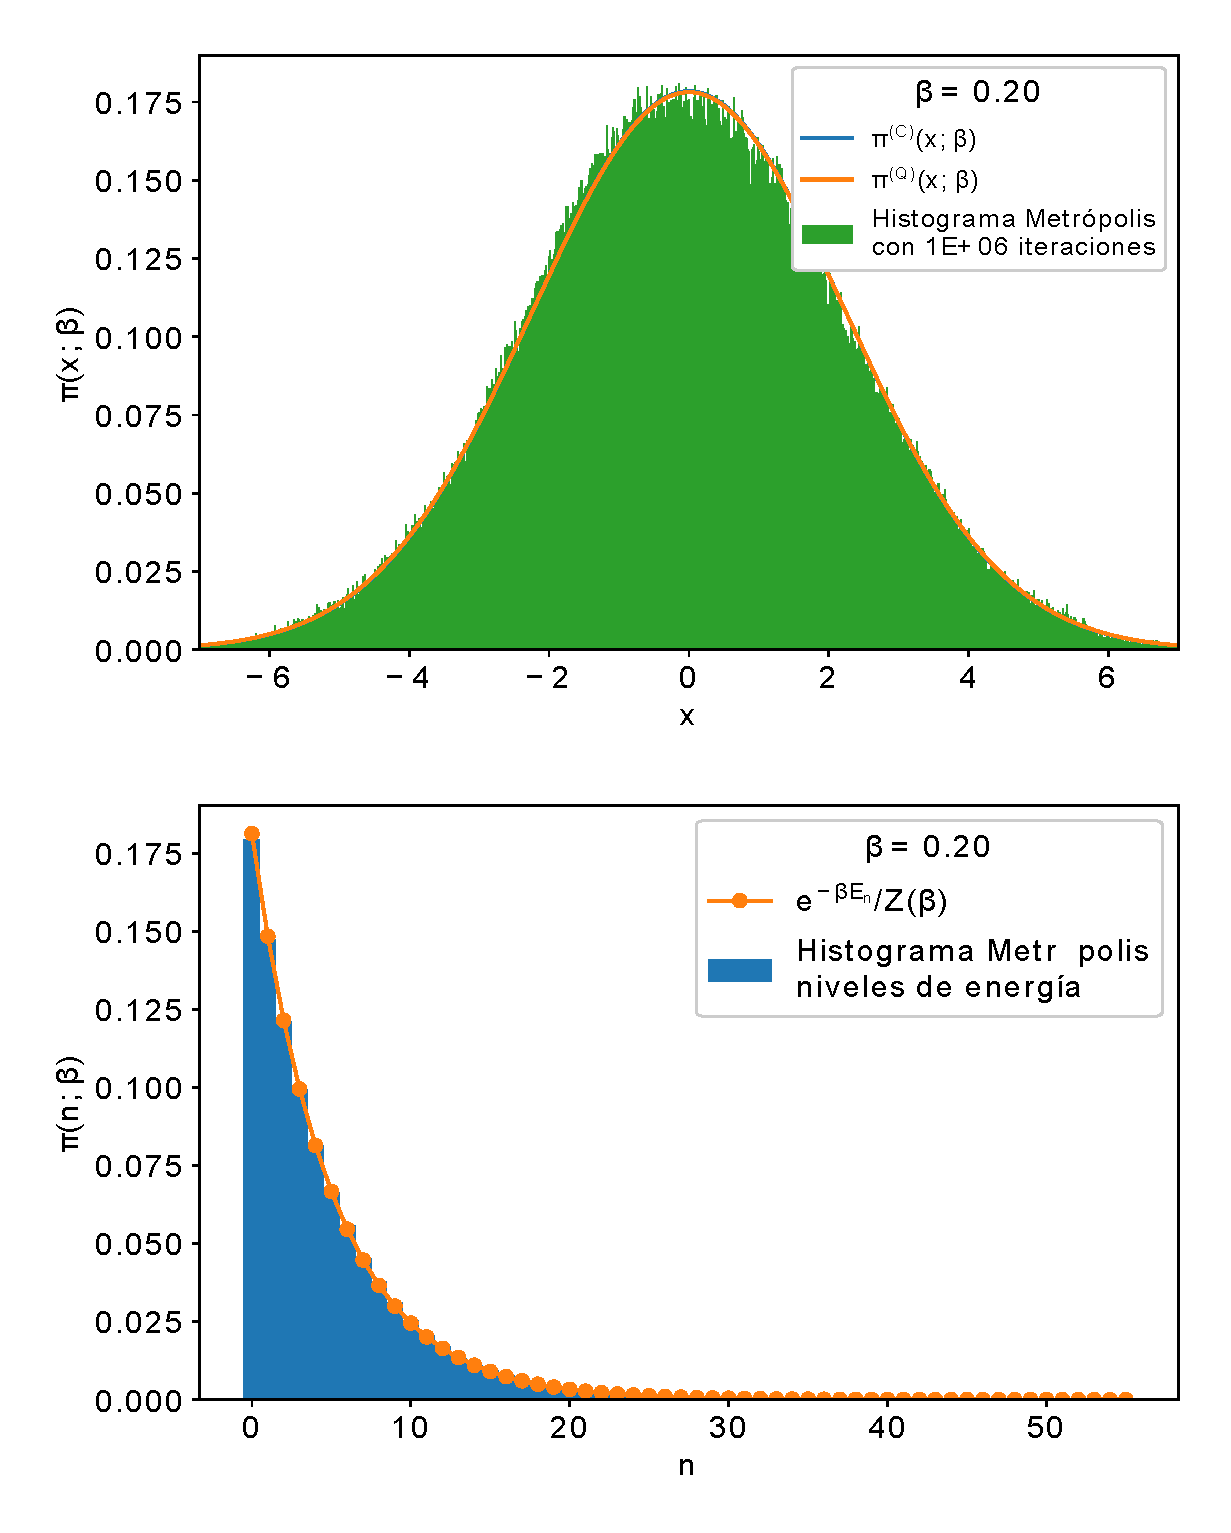
\includegraphics[width=\linewidth]{figures/0_plot_QHO_finite_temp_beta_0_20}
	\caption{Arriba: densidad de probabilidad de encontrar a la «partícula» cuántica en una posición dada, cuando está en presencia de un potencial armónico y de baño térmico a temperatura definida por $\beta=1/T=0.2$. Mostramos los resultados teóricos clásico y cuántico como línea continua y el histograma que resulta del algoritmo Metrópolis usando $10^6$ iteraciones y $\delta x = 0.5$. Observamos que éste es un límite de alta temperatura ya que las distribuciones teóricas clásica y cuántica se solapan en gran medida y son muy similares. Abajo: histograma de niveles de energía obtenido con algoritmo Metrópolis y los respectivos valores teóricos. Notamos que muchos niveles de energía contribuyen en este caso que hemos considerado de alta temperatura. Además, los valores calculados por el algoritmo se acercan en gran medida a los teóricos}
	\label{fig:beta_0.2}
\end{figure}

El caso $\beta=1.0$ que se ilustra en la figura \ref{fig:beta_1.0} es un caso intermedio entre el límite de alta y baja temperatura. Aquí podemos observar perfectamente, aunque no muy grande, la diferencia entre los resultados teóricos clásico y cuántico. Encontramos también que el algoritmo Metrópolis hace bien el trabajo y se aproxima mejor a la densidad de probabilidad cuántica teórica, $\pi^{(Q)}(x;\beta)$. Aquí, el histograma para los niveles de energía generado por el algoritmo se acerca más a (\ref{eq:pi-energy-levels}) y notamos que el número de niveles de energía que contribuyen significativamente es menor en este caso que en el caso $\beta=0.2$ (figura \ref{fig:beta_0.2}) por un factor de aproximadamente 4.

\begin{figure}[!b]
	\centering
	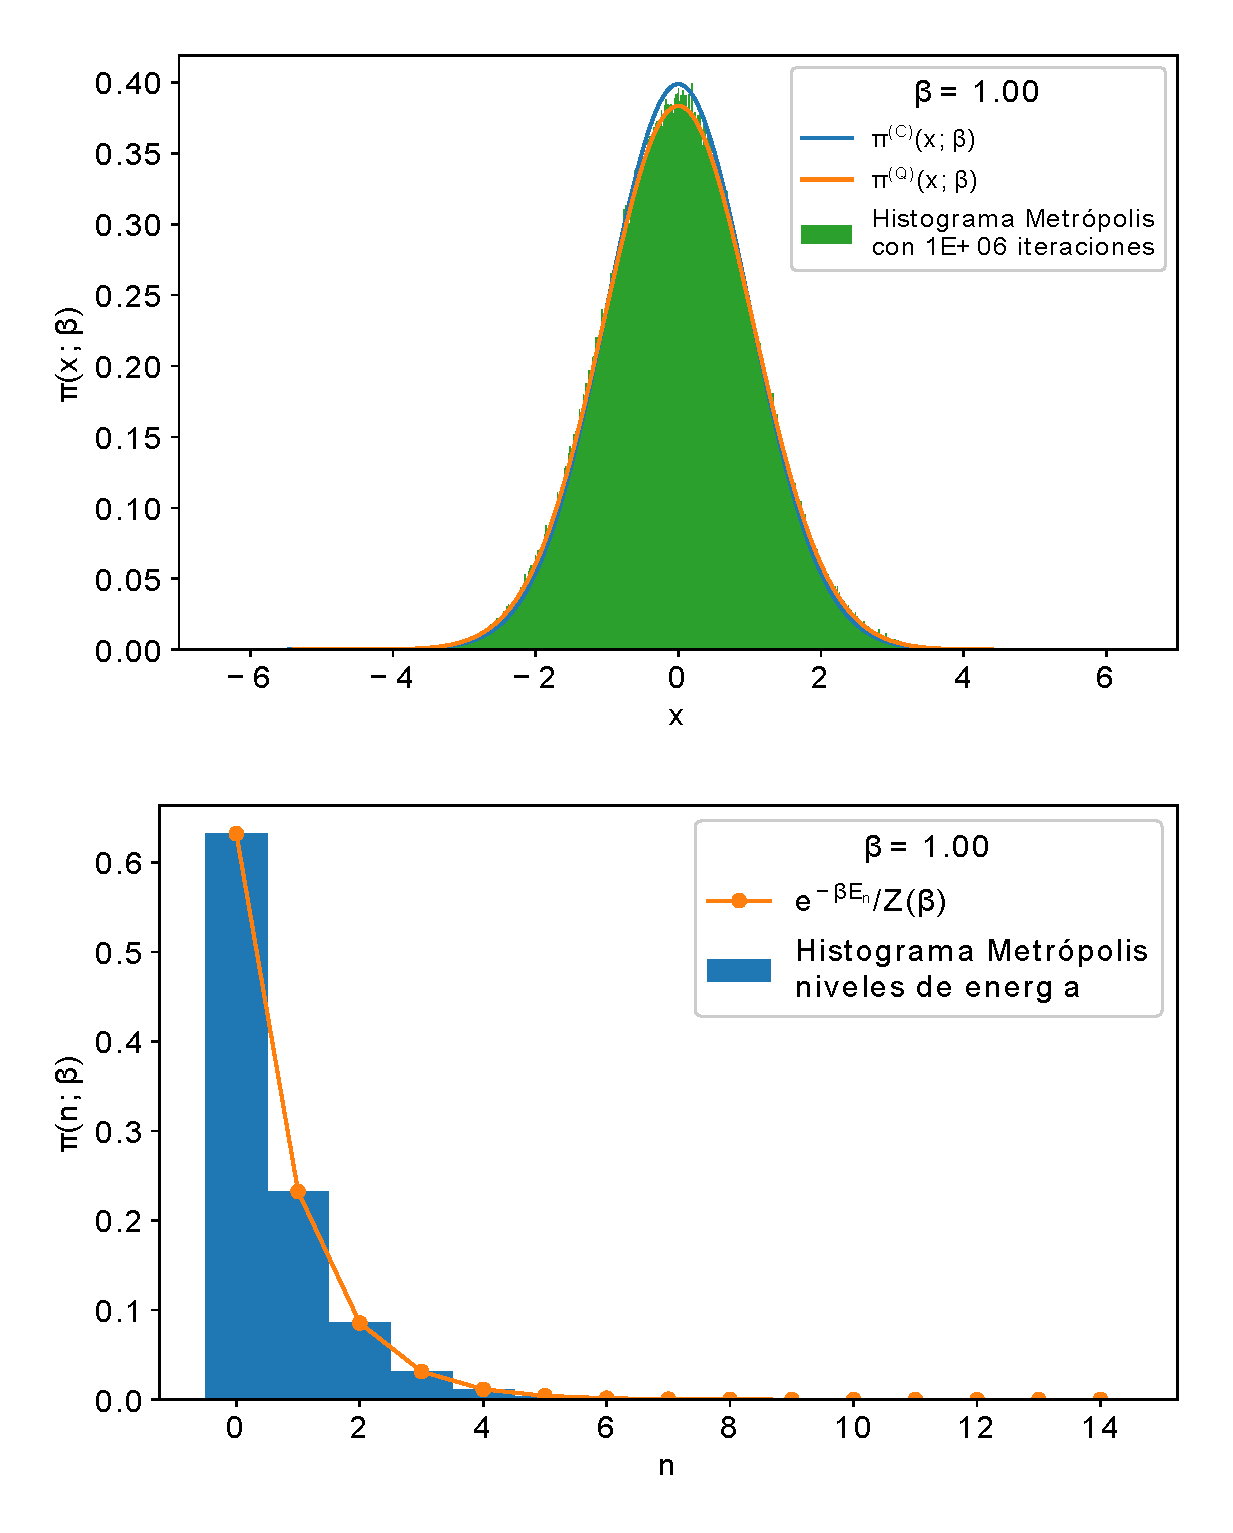
\includegraphics[width=\linewidth]{figures/0_plot_QHO_finite_temp_beta_1_0}
	\caption{Arriba: densidad de probabilidad de encontrar a la «partícula» cuántica en una posición dada, cuando está en presencia de un potencial armónico y de baño térmico a temperatura definida por $\beta=1/T=1.0$. Mostramos los resultados teóricos clásico y cuántico como línea continua y el histograma que resulta del algoritmo Metrópolis usando $10^6$ iteraciones y $\delta x = 0.5$. Observamos que éste es un caso intermedio entre los límites de alta y baja temperatura ya que las distribuciones teóricas clásica y cuántica son evidentemente diferentes aunque aún tengan cierta similitud (en los valores exactos para cada $x$ la similitud es del orden del $90\%$). Abajo: histograma de niveles de energía obtenido con algoritmo Metrópolis y los respectivos valores teóricos marcados con puntos. Este caso de temperatura media entre límite de alta y baja temperatura tiene contribuciones de muchos menos niveles de energía que el caso $\beta=0.2$, el cual es de baja temperatura. Los valores obtenidos con el algoritmo se acercan mucho a los valoresteóricos marcados por los puntos.}
	\label{fig:beta_1.0}
\end{figure}

Finalmente, en la figura \ref{fig:beta_5.0} vemos un caso de baja temperatura, $\beta=5$, pero evidentemente no en el cero absoluto. Aquí las diferencias entre la distribución cuántica y la clásica son muy notorias y la distribución clásica tiene una desviación estandar más pequeña que la cuántica. Recordemos que conforme la temperatura baja, el caso clásico tiende a una desviación estandar de cero \textit{i.e.} a una delta de Dirac. En este caso, al igual que los anteriores, el algoritmo de metrópolis muestrea correctamente la probabilidad cuántica. Aquí notamos en el histograma para $n$ que hay una disminución importante en el número de niveles de energía que contribuyen significativamente en el sistema. Prácticamente el nivel dominante es $E_0$ que corresponde al estado base del sistema, que corresponde a un límite de baja temperatura, en conformidad con lo que analizamos anteriormente para el histograma de posiciones.

\begin{figure}[t]
	\centering
	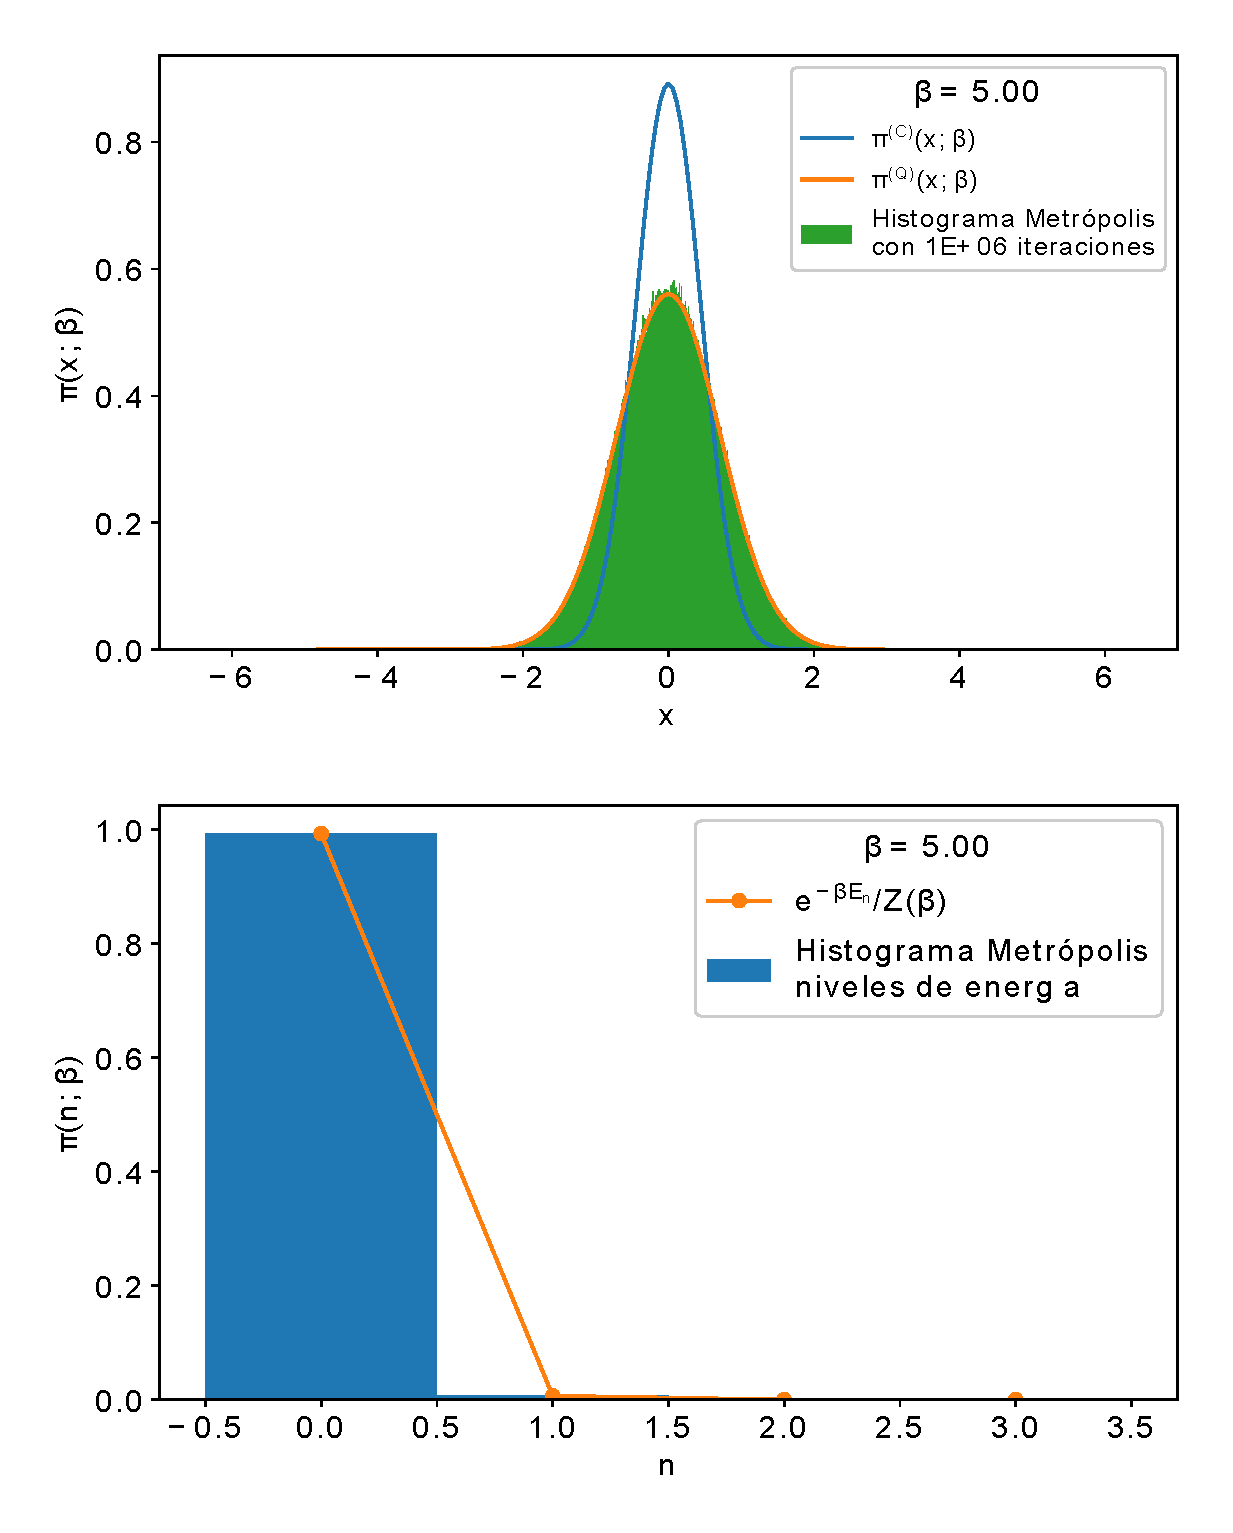
\includegraphics[width=\linewidth]{figures/0_plot_QHO_finite_temp_beta_5_0}
	\caption{Arriba: densidad de probabilidad de encontrar a la «partícula» cuántica en una posición dada, cuando está en presencia de un potencial armónico y de baño térmico a temperatura definida por $\beta=1/T=5.0$. Mostramos los resultados teóricos clásico y cuántico como línea continua y el histograma que resulta del algoritmo Metrópolis usando $10^6$ iteraciones y $\delta x = 0.5$. Observamos que éste es un límite de baja temperatura ya que las distribuciones teóricas clásica y cuántica son muy diferentes en sus valores específicos, a diferencia de lo notado en las figuras \ref{fig:beta_0.2} y \ref{fig:beta_1.0}. Abajo: histograma de niveles de energía obtenido con algoritmo Metrópolis y los respectivos valores teóricos marcados con puntos. Aquí el histograma ya está comprendido por los niveles de energía más bajos, lo cual corresponde con el límite de baja temperatura. El nivel que más contribuye evidentemente es el estado base y los valores obtenidos con el algoritmo se ajustan casi perfectamente a los teóricos.}
	\label{fig:beta_5.0}
\end{figure}

En cuanto al tiempo de cómputo del algoritmo, éste depende del valor de $\beta$. Conforme $\beta$ disminuye (se consideran mayores temperaturas), el tiempo de cómputo aumenta ya que el sistema puede acceder a niveles de energía más altos. En el algoritmo ésto se traduce en que se deben computar los valores de $\psi_n$ para todos los valores de $x$ considerados hasta el momento, esto es, que hacen parte de la lista con la que se construye el histograma. En este punto tal vez el algoritmo pueda ser optimizado para reducir el tiempo de cómputo, ingeniando una manera de no tener que calcular $\psi_n$ para todos los valores de $x$ considerados, sino solo para los que necesiten ser usados. En nuestro caso (lo relevante más que los tiempos de cómputo son las proporciones entre dichos tiempos) el algoritmo demora aproximadamente $190s$ para el caso $\beta = 0.2$, $110s$ para $\beta = 1.0$ y $80s$ para $\beta=5.0$. En el caso de $T=0$ que simplificamos al muestreo de la distribución de probabilidad $\left|\psi_0(x)\right|^2$ y que tratamos en la sección \ref{subsec:limite-T-0}, el algoritmo demora aproximadamente de $20s$.

En cuanto a la convergencia del algoritmo a la distribución de probabilidad cuántica $\pi^{(Q)}(x;\beta)$, hay que mencionar que aunque no está reportado acá en gráficas, si se puede verificar que para valores más pequeños de $\beta$ (manteniendo $\delta x$ constante) el algoritmo necesita más iteraciones para converger a la densidad de probabilidad dada —en cierta medida esto se puede ver si ampliamos un poco las figuras \ref{fig:beta_0.2}, \ref{fig:beta_1.0} y \ref{fig:beta_5.0} ya que conforme disminuye $\beta$, las fluctuaciones en el histograma son mayores. El motivo de esto es similar al dado anteriormente: para temperaturas más altas, el sistema puede acceder a niveles de energía más altos. Esto se traduce a que se deben muestrear posiciones más alejadas de la región de mayor probabilidad ya que el acceso a niveles de energía mayores implica en últimas que la desviación estandar aumenta conforme aumenta la temperatura. En este caso se podría optimizar el algoritmo haciendo un análisis juicioso del valor de $\delta x$ necesario para muestrear los posibles valores de $x$ de manera más eficiente.

Como comentario final de esta sección, es importante también mencionar que los algoritmos se ejecutaron en Python3 v3.6.

\section{Conclusión\label{sec:conclusion}}

En este trabajo estudiamos el problema del oscilador armónico en un baño térmico, tanto de forma clásica como cuántica y con un tratamiento teórico y computacional –éste último en el marco del algoritmo Metrópolis.

Pudimos calcular para el oscilador armónico cuántico en un baño térmico los elementos diagonales del operador densidad en la base de posiciones, $\rho(x,x;\beta)$. Estos elementos diagonales los interpretamos como la densidad de probabilidad de encontrar a la «partícula» en la posición $x$: $\pi^{(Q)}(x;\beta)$. En el caso clásico calculamos esta probabilidad con ayuda de la función de distribución en el espacio de fase definida por el ensamble canónico. Encontramos que el límite de baja temperatura para el caso clásico es una delta de Dirac centrada en el origen, mientras que en el caso cuántico este límite corresponde con la densidad de probabilidad de la autofunción de energía del estado base del oscilador armónico, conforme se espera. De igual modo pudimos notar que en el límite de altas temperaturas la densidad de probablididad cuántica mencionada tiende a la clásica, conforme se espera también desde la física estadística. 

Para contrastar los resultados teóricos usamos el algoritmo Metrópolis para reconstruir los histogramas del sistema cuántico en el espacio de las posiciones y en los niveles de energía. Para los casos de $\beta$ evaluados encontramos que uno corresponde a un límite de alta temperatura ya que las distribuciones cuántica y clásica eran muy parecidas, también tenemos un caso intermedio entre alta y baja temperatura y uno de baja temperatura. Esas conclusiones las soportamos tanto en las comparaciones de las curvas teóricas como en los histogramas generados. Siempre los histogramas de los niveles de energía corresponden con el límite que tratamos: altas temperaturas implican contribuciones apreciables de muchos niveles de energía, mientras que para bajas temperaturas contribuyen solo niveles muy próximos al estado base.

Las implementaciones de los algoritmos usados son suficientemente generales y se podrían adaptar con cierta facilidad a otros sistemas de interés que sean objeto de estudio.

\section*{Agradecimientos}
Agradezco a mis compañeros de clase con los que tuve discusiones que ayudaron en la implementación del algoritmo y en las conclusiones presentadas. 

\nocite{*}

\bibliography{5-Semestre_X_2020_I-Fisica_Estadistica_Avanzada-Tarea_1}% Produces the bibliography via BibTeX.

\newpage



\appendix

\begin{widetext}

\section{Código 1: Oscilador Armónico Cuántico a muy baja temperatura \texorpdfstring{$T \rightarrow 0$}{T tendiendo a cero}\label{appx:codigo_baja_temperatura}}

\inputminted[linenos,breaklines]{python}{code_1.py}

\section{Código 2: Oscilador Armónico Cuántico a temperatura finita \texorpdfstring{$T \neq 0$}{T diferente de cero}\label{appx:codigo_temperatura_finita}}

\inputminted[linenos,breaklines]{python}{code_2.py}

\end{widetext}


\end{document}
%
% ****** End of file apssamp.tex ******
